\documentclass{ximera}



% MATH -----------------------------------------------------------
\newcommand{\nats}{\mathbb N}
\newcommand{\ints}{\mathbb Z}
\newcommand{\rats}{\mathbb Q}
\newcommand{\reals}{\mathbb R}
\newcommand{\complex}{\mathbb C}
\newcommand{\powerset}{\mathscr P}

%-------------------------------------------------------------


\begin{document}
\begin{abstract}
 \end{abstract}

    \title{First Order Applications, Part II}
    
    \maketitle


 There are many applications of the theory of first order differential equations.  We continue with another sampling of applications.\\


 \emph{Motion with resistance}:   When an object is traveling vertically through a medium (air or water for example) a constant gravitational force pulls the object down, but the medium also exerts resistance, sometimes modeled as directly proportional to the speed of the object.\\

 Let's derive an IVP for vertical motion with such resistance.  \\

 Let $v(t)$ be the velocity at time $t$ of an object of mass $m>0$ moving vertically through a medium.  There is a constant downward gravitational force of magnitude $F_{g}=mg$ (where $g>0$ is the constant acceleration due to gravity).  If we don't ignore medium resistance, we might model the resistive force of a medium as having magnitude $F_{m}=k|v|$ (where $k>0$ depends on the medium and object) in the \emph{opposite direction of the motion}, where $v$ is the velocity of the object.\\

 Using the upward direction as positive we write that $F_g=-mg$ and $F_m=-kv$, noting that when $v<0$ the resistive force should be positive and when $v>0$ the resistive force should be negative.  Newton's second law of motion asserts that the sum of all forces is equal to $ma$, where a is the acceleration.  Sometimes we write $\displaystyle \sum F=mv'$.\\

 Putting this all together we get \framebox{ $mv'=-mg-kv$, $v(0)=v_0$} using $t=0$ for the initial time and $v_0$ for the initial velocity.\\

 This can be re-expressed as $v'=-g-\dfrac{k}{m}v$.  This both separable and linear, so you should know two ways to solve this!\\

%%%%%%%%%%%%%%%%%%%%%%%%%%%%%%%%%%%%%%%%%%%%
% I'd suggest pausing the video and practicing!
%%%%%%%%%%%%%%%%%%%%%%%%%%%%%%%%%%%%%%%%%%%%

\newpage

 Solving it as a separable equation yields either $v=-\frac{mg}{k}$ (equilibrium solution) or  \\

 $v'=-g-\dfrac{k}{m}v\rightarrow \;$ $\displaystyle \frac{1}{-g-\frac{k}{m}v}v'=1\rightarrow \;$ $\displaystyle -\frac{m}{k}\ln{\left|-g-\frac{k}{m}v\right|}=t+C\rightarrow $ \\

 $\displaystyle \ln{\left|-g-\frac{k}{m}v\right|}=-\frac{k}{m}t+C\rightarrow \;$  $\displaystyle -g-\frac{k}{m}v=Ce^{-\frac{k}{m}t}\rightarrow \;$  $\displaystyle v=-\frac{mg}{k}+Ce^{-\frac{k}{m}t}$, and since $v(0)=v_0$, \\

 $\displaystyle v=-\frac{mg}{k}+\left(v_0+\frac{mg}{k}\right)e^{-\frac{k}{m}t}$.\\

 A couple observations:  This solution includes the equilibrium solution $v=-\frac{mg}{k}$.  All solutions $v$ satisfy $\displaystyle \lim_{t\rightarrow \infty}v(t)$ $=-\frac{mg}{k}$.  We call $v_t=-\frac{mg}{k}$ the $``$terminal velocity" of the object. \\ \\



Example:   Suppose a 192 lb person dives from a helicopter vertically toward the surface of the Earth.   Assume that the air resists the motion of the skydiver with a force proportional to the speed of the skydiver  and that the skydiver approaches a terminal speed of $176$ feet per second.   Find the velocity of the skydiver at $t$ seconds into the skydive (for the time of flight before the parachute is deployed).  If after $20$ seconds, the skydiver pulls the parachute, then determine the speed at this moment.\\

 We must remember here that pounds are units of force (gravitational weight $mg$).  So in particular, the mass of the person is $m=192/32=6$ (slugs) using $g=32$ feet per second-squared for the acceleration due to gravity.\\

 Since we have that the terminal velocity is $v_t=-176=-\frac{mg}{k}$, we can solve for the constant of proportionality of medium resistance:  $k=\frac{192}{176}\approx 1.09$.  We can use the model on the previous page, and that $v(0)=0$ to get $\displaystyle v(t)\approx -176+176e^{-(1.09/6)t}\approx -176\left(1-e^{-0.18 t}\right)$.  So $|v(20)|\approx 171$ ft/s (about 117 mph).

 Exercise left for you:  If the sky diver pulled the parachute at 600 ft from the surface of the Earth, then at what height was the helicopter?\\ \\

%%%%%%%%%%%%%%%%%%%%%%%%%%%%%%%%%%%%%%%%%%%
% You should get 3200 ft to the nearest 100 ft.
%%%%%%%%%%%%%%%%%%%%%%%%%%%%%%%%%%%%%%%%%

\newpage


 \emph{Escape Velocity}:  Over larger vertical distances, gravitational models must reflect that the \emph{gravitational force exerted by the Earth on an object is actually inversely proportional to the square of the distance from the center of Earth}. \\

 Assume a spacecraft launches from the surface of the Earth and exhausts its launch fuel as it reaches a height $h$ that sufficiently large so that atmospheric resistance is negligible and can be assumed to be effectively $0$. \\

 Let $t=0$ be this time (known as $``$burnout") and consider that the force of gravity on the spacecraft at altitude $y\geq h$ is $\displaystyle F_{g}=-\frac{c}{(R+y)^{2}}$ where $c$ is a constant and $R$ is the radius of the Earth.\\

\begin{figure}[h]
\centering
 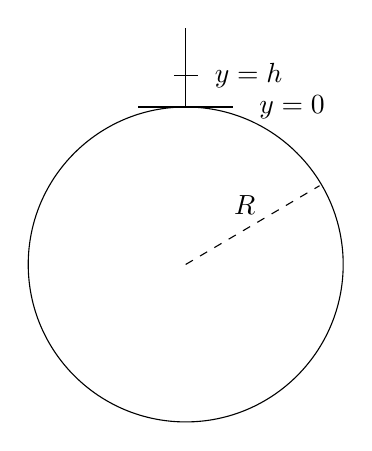
\begin{tikzpicture}[scale=1]
 \draw (0,0) circle (2);
 \draw (0,2) -- (0,3);
  \draw (-0.6,2) node at (1.35,2) {$y=0$} -- (0.6,2);
 \draw (-0.15,2.4) node at (0.8,2.4) {$y=h$} -- (0.15,2.4);
 \draw[dashed] (0,0) node at (0.75,0.75) {$R$} -- (1.7,1);
 \end{tikzpicture}
 \caption{Escape velocity diagram}
 \end{figure}


 Using $F_{g}=-mg$ when $y=0$ where $m$ is the mass of the spacecraft (assume the mass of the launch fuel is negligible compared to the mass of the spacecraft) and $g$ is the acceleration due to gravity on the surface of the Earth, we get $-mg=-\frac{c}{R^{2}}$, so $c=mgR^{2}$.\\


 Thus $\displaystyle F_{g}=-\frac{mgR^{2}}{(R+y)^{2}}$.   Since $F_{g}$ is assumed to be the only force acting on the spacecraft for $t\geq 0$, $\displaystyle F_{g}=ma=my''=-\dfrac{mgR^{2}}{(R+y)^{2}}\rightarrow $   $\displaystyle y''=-\dfrac{gR^{2}}{(R+y)^{2}}$.\\


 This equation is an example of a $``$second order autonomous" equation (where $y''=f(y,y')$ doesn't involve the independent input variable).   We can transform it into a first order de involving velocities: Let $v(y)$ be the vertical velocity at altitude $y$.   By the chain rule, $\displaystyle \frac{d^{2}y}{dt^{2}}=\frac{dv}{dt}=\frac{dv}{dy}\frac{dy}{dt}=v\frac{dv}{dy}$.\\


 Now we solve the de $\displaystyle v\frac{dv}{dy}=-\frac{gR^{2}}{(R+y)^{2}}$.  This equation is separable, and integrating both sides yields  \\ $\displaystyle 0.5v^{2}=\frac{gR^{2}}{R+y}+C\rightarrow$ $\displaystyle v(y)=\sqrt{\frac{2gR^{2}}{R+y}+C}$.\\


 Now suppose we have a burnout velocity of $v(h)=v_{0}$. Then $v_{0}^{2}=\dfrac{2gR^{2}}{R+h}+C$.\\

 So $C=v_{0}^{2}-\dfrac{2gR^{2}}{R+h}$  and hence $\displaystyle v=\sqrt{\frac{2gR^{2}}{R+y}+v_{0}^{2}-\dfrac{2gR^{2}}{R+h}}$.\\


 If $v_{0}\geq \sqrt{\dfrac{2gR^{2}}{R+h}}$ then $v\geq 0$ for all $y\geq h$ and the spacecraft continues on up into space!  Otherwise one can show (see below) that the spacecraft is pulled back towards Earth.\\

The expression $v_{e}=\sqrt{\dfrac{2gR^{2}}{R+h}}$ is called \underline{escape velocity}.\\

 If $\displaystyle v_{0} < \sqrt{\frac{2gR^2}{R+h}}$ then $\displaystyle v_{0}^{2} < \frac{2gR^2}{R+h}$ and hence $\displaystyle v(y)=\sqrt{\frac{2gR^2}{R+y}-\left[\frac{2gR^2}{R+h}-v_{0}^{2}\right]}=0$ for a value of $y$ such that $\displaystyle \frac{2gR^2}{R+y} = \frac{2gR^2}{R+h} - v_{0}^{2} < \frac{2gR^2}{R+h}$, implying that $R+y>R+h$, or equivalently $y>h$. And if $v(y)=0$ for some value of $y>h$, the spacecraft will be pulled back towards Earth by gravity. 


\end{document}